\documentclass[12pt]{article}
\usepackage[spanish]{babel}
\usepackage{geometry}
\geometry{a4paper, margin=1in}
\usepackage{graphicx}
\usepackage{xcolor}
\usepackage{titlesec}
\usepackage{parskip}
\usepackage{multicol}
\usepackage{cite}
\usepackage{float}
\usepackage{amsmath}


\definecolor{highlight}{RGB}{255, 255, 0}

\titleformat{\section}{\normalfont\Large\bfseries}{\thesection}{1em}{}
\titleformat{\subsection}{\normalfont\large\bfseries}{\thesubsection}{1em}{}

\begin{document}

% Logos
\begin{minipage}{0.45\textwidth}
    
\includegraphics[width=0.4\textwidth]{inFiles/Figures/epnLogo.jpg}
\end{minipage}
\hfill
\begin{minipage}{0.45\textwidth}
    \raggedleft
    
\includegraphics[width=0.4\textwidth]{inFiles/Figures/FIS_logo.jpg}
\end{minipage}

\vspace{0.5cm}

% Títulos principales
\begin{center}
    \textbf{ESCUELA POLITÉCNICA NACIONAL}\\[0.2cm]
    \textbf{FACULTAD DE INGENIERÍA DE SISTEMAS}\\[0.2cm]
    \textbf{INGENIERÍA {\textbf{EN COMPUTACIÓN}}}
\end{center}

\vspace{0.5cm}
\hrule
\vspace{0.5cm}

% Datos principales
\noindent\textbf{PERÍODO ACADÉMICO:} 2025-A\\[0.2cm]
\noindent\textbf{ASIGNATURA:} ICCD412 Métodos Numéricos \hfill \textbf{GRUPO:} GR2\\[0.2cm]
\noindent\textbf{TIPO DE INSTRUMENTO:} Tarea 12\\[0.2cm]
\noindent\textbf{FECHA DE ENTREGA LÍMITE:} 29/06/2025\\[0.2cm]
\noindent\textbf{ALUMNO:} Murillo Tobar Juan

\vspace{0.5cm}
\hrule
\vspace{1cm}


% Secciones
\section*{TEMA}
Eliminación Gaussiana y Gauss-Jordan

\vspace{0.5cm}

\section*{OBJETIVOS}
\begin{itemize}
    \item Utilizar el método de Gauss para la  resolución de sistemas de ecuaciones lineales.
    \item Utilizar el método de Gauss Jordan para la resolución de sistemas de ecuaciones lineales.

\end{itemize}

\vspace{0.5cm}


\section*{DESARROLLO}

\begin{figure}[H]
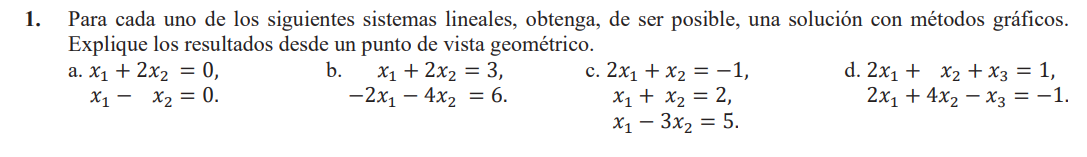
\includegraphics[width=1\textwidth]{./inFiles/Figures/Ej1.png}
\end{figure}

\textbf{a)}
\begin{figure}[H]
\centering
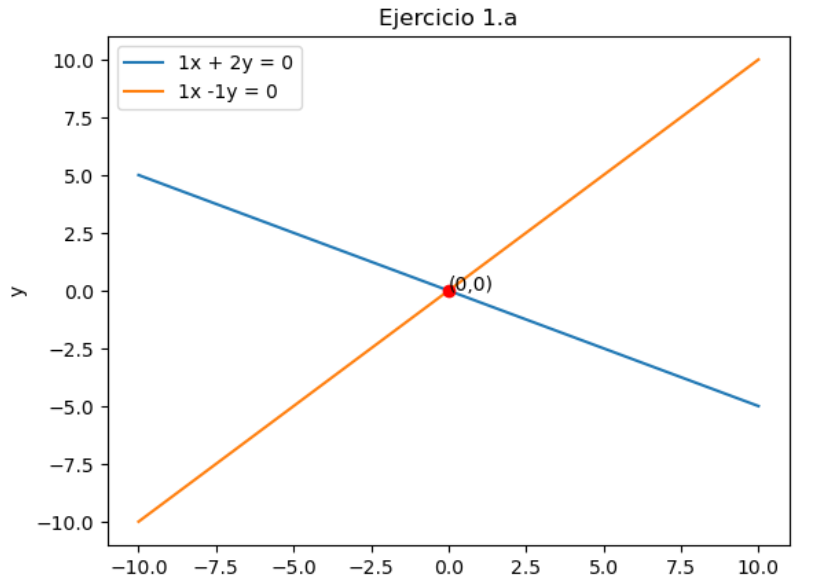
\includegraphics[width=0.7\textwidth]{./inFiles/Figures/Ej1a.png}
\end{figure}
En este caso se obtuvo una solución ya que existe un punto en común entre ambas rectas.
\textbf{b)}
\begin{figure}[H]
\centering
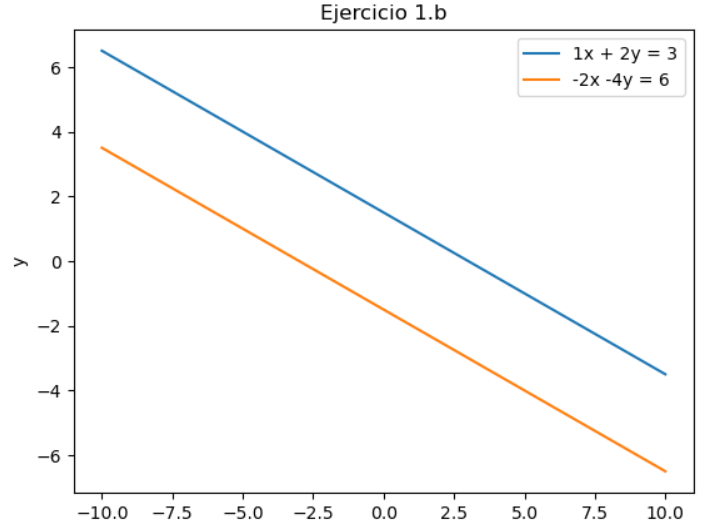
\includegraphics[width=0.7\textwidth]{./inFiles/Figures/Ej1b.png}
\end{figure}
No existen soluciones porque ambas rectas son paralelas y no se cortaran en un punto.
\newpage
\textbf{c)}
\begin{figure}[H]
\centering
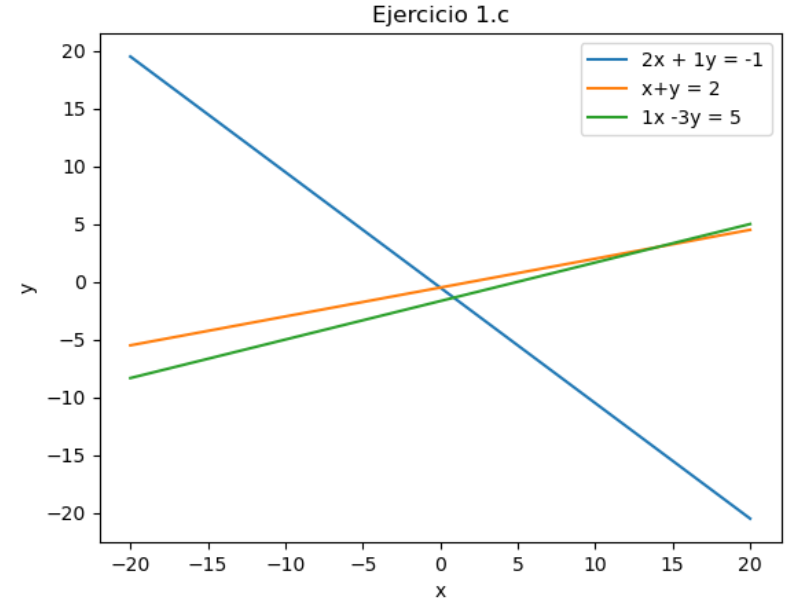
\includegraphics[width=0.7\textwidth]{./inFiles/Figures/Ej1c.png}
\end{figure}
No existe ni única solución ni infinitas soluciones porque no tienen un punto de corte en común.

\textbf{d)}
\begin{figure}[H]
\centering
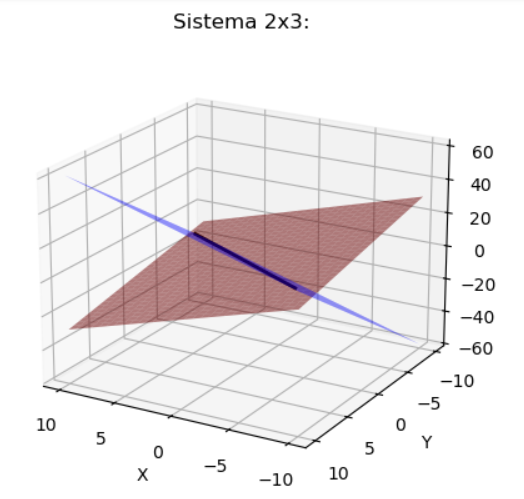
\includegraphics[width=0.7\textwidth]{./inFiles/Figures/Ej1d.png}
\end{figure}

Existen infinitas soluciones porque ambos planos se cortan formando una recta con infinitos puntos.


\begin{figure}[H]
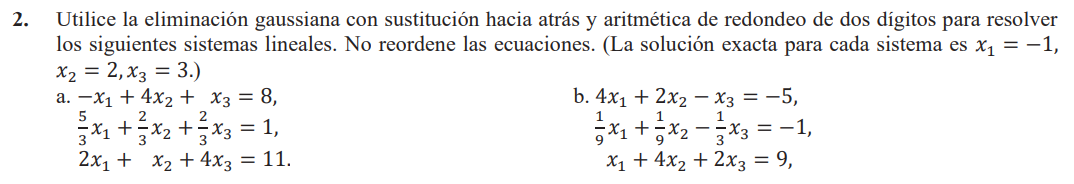
\includegraphics[width=1\textwidth]{./inFiles/Figures/Ej2.png}
\end{figure}

\textbf{a)}
\[
\begin{bmatrix}
-1 & 4 & 1 & 8 \\
1.67 & 0.67 & 0.67 & 1 \\
2 & 1 & 4 & 11
\end{bmatrix}
\]
1.67*F1+F2 $\longrightarrow $ F2

2*F1+F3 $\longrightarrow $ F3

\[
\begin{bmatrix}
-1 & 4 & 1 & 8 \\
0 & 7.35 & 2.34& 14.36 \\
0 & 9 & 6 & 27
\end{bmatrix}
\]

9*F2-7.35*F3 $\longrightarrow $ F3

\[
\begin{bmatrix}
-1 & 4 & 1 & 8 \\
0 & 7.35 & 2.34& 14.36 \\
0 & 0 & -23.04 & -69.21
\end{bmatrix}
\]

Haciendo la substitución para atrás Y redondeando obtenemos
$X3 = 3.00$    $X2 =1.00$  $X1 =-1.00$ 

\textbf{b)}
\[
\begin{bmatrix}
4 & 2 & -1 & -5 \\
0.11 & 0.11 & -0.33 & -1 \\
1 & 4 & 2 & 9
\end{bmatrix}
\]
-0.11*F1+4*F2 $\longrightarrow $ F2

-4*F3+F1 $\longrightarrow $ F3

\[
\begin{bmatrix}
4 & 2 & -1 & -5 \\
0 & 0.22 & -1,21& -3.45 \\
0 & -14 & -9 & -41
\end{bmatrix}
\]

14*F2+0.22*F3 $\longrightarrow $ F3

\[
\begin{bmatrix}
4 & 2 & -1 & -5 \\
0 & 0.22 & -1,21& -3.45 \\
0 & 0 & -18.92 & -57.32
\end{bmatrix}
\]

Haciendo la substitución para atrás Y redondeando obtenemos
$X3 = 3.03$    $X2 =0.98$  $X1 =-0.98$ 


\begin{figure}[H]
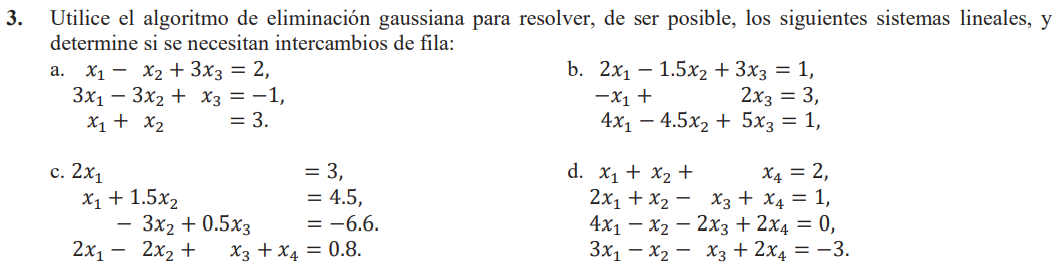
\includegraphics[width=1\textwidth]{./inFiles/Figures/Ej3.png}
\end{figure}

Por código:
\begin{figure}[H]
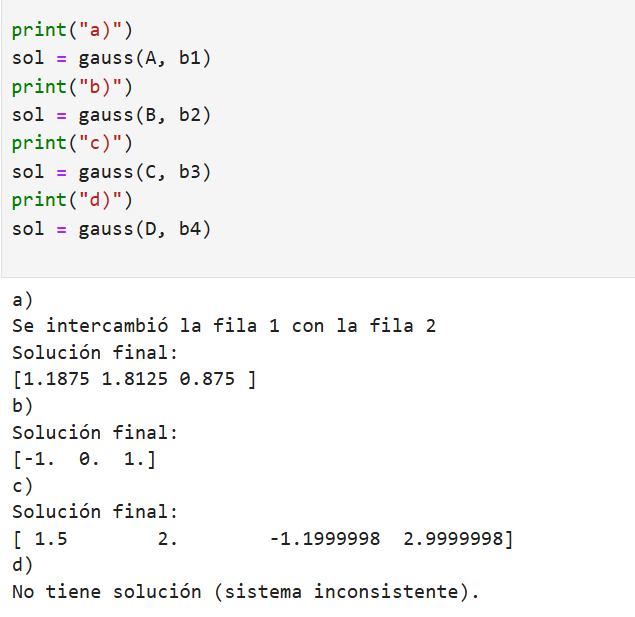
\includegraphics[width=1\textwidth]{./inFiles/Figures/PC3.png}
\end{figure}

A mano:

\textbf{a)}
\[
\begin{bmatrix}
1 & -1 & 3 & 2 \\
3 & -3 & 1& -1 \\
1 & 1 & 0 & 3
\end{bmatrix}
\]

-3*F1+F2 $\longrightarrow $ F2

-F1+F3 $\longrightarrow $ F3

\[
\begin{bmatrix}
1 & -1 & 3 & 2 \\
0 & 0 & -8& -7 \\
0 & 2 & -3 & 1
\end{bmatrix}
\]

F3 cambia con F2 (Si hubo cambio de filas)

\[
\begin{bmatrix}
1 & -1 & 3 & 2 \\
0 & 2 & -3 & 1 \\
0 & 0 & -8 & -7
\end{bmatrix}
\]

Haciendo la substitución para atrás Y redondeando obtenemos
$X3 = 0.875$    $X2 =1.8125$  $X1 =1.1875$ 

\textbf{b)}
\[
\begin{bmatrix}
2 & -1.5 & 3 & 1 \\
-1 & 0 & 2& 3 \\
4 & -4.5 & 5 & 1
\end{bmatrix}
\]

F1+2*F2 $\longrightarrow $ F2

-2*F1+F3 $\longrightarrow $ F3

\[
\begin{bmatrix}
2 & -1.5 & 3 & 1 \\
0 & -1.5 & 7& 7 \\
0 & -1.5 & -1 & -1
\end{bmatrix}
\]

-F2+F3 $\longrightarrow $ F3

\[
\begin{bmatrix}
2 & -1.5 & 3 & 1 \\
0 & -1.5 & 7& 7 \\
0 & 0 & -8 & -8
\end{bmatrix}
\]

(No hubo cambio de filas)

Haciendo la substitución para atrás Y redondeando obtenemos
$X3 = 1$    $X2 =0$  $X1 =-1$ 

\textbf{c)}
\[
\begin{bmatrix}
2 & 0 & 0 & 0 & 3 \\
1 & 1.5 & 0& 0& 4.5 \\
0 & -3 & 0.5 & 0 & -6.6 \\
2 & -2 & 1 & 1 & 0.8 \\
\end{bmatrix}
\]

-2F2+F1 $\longrightarrow $ F2

-F1+F4 $\longrightarrow $ F4

\[
\begin{bmatrix}
2 & 0 & 0 & 0 & 3 \\
0 & -3 & 0& 0& -6 \\
0 & -3 & 0.5 & 0 & -6.6 \\
0 & -2 & 1 & 1 & -2.2 \\
\end{bmatrix}
\]

-F2+F3 $\longrightarrow $ F3

-2F2+3F4 $\longrightarrow $ F4

\[
\begin{bmatrix}
2 & 0 & 0 & 0 & 3 \\
0 & -3 & 0& 0& -6 \\
0 & 0 & 0.5 & 0 & -0.6 \\
0 & 0 & 3 & 3 & 5.4 \\
\end{bmatrix}
\]

-6F3+F4 $\longrightarrow $ F4

\[
\begin{bmatrix}
2 & 0 & 0 & 0 & 3 \\
0 & -3 & 0& 0& -6 \\
0 & 0 & 0.5 & 0 & -0.6 \\
0 & 0 & 0 & 3 & 9 \\
\end{bmatrix}
\]

(No hubo cambio de filas)

Haciendo la substitución para atrás Y redondeando obtenemos
$X4 = 3$   $X3 = -1.2$   $X2 =2$  $X1 =1.5$ 

\textbf{d)}
\[
\begin{bmatrix}
1 & 1 & 0 & 1 & 2 \\
2 & 1 & -1& 1& 1 \\
4 & -1 & -2 & 2 & 0 \\
3 & -1 & -1 & 2 & -3 \\
\end{bmatrix}
\]

-2F1+F2 $\longrightarrow $ F2

-4F1+F3 $\longrightarrow $ F3

-3F1+F4 $\longrightarrow $ F4

\[
\begin{bmatrix}
1 & 1 & 0 & 1 & 2 \\
0 & -1 & -1& -1& -3 \\
0 & -5 & -2 & -2 & -8 \\
0 & -4 & -1 & -1 & -9 \\
\end{bmatrix}
\]

-5F2+F3 $\longrightarrow $ F3

-4F2+3F4 $\longrightarrow $ F4

\[
\begin{bmatrix}
1 & 1 & 0 & 1 & 2 \\
0 & -1 & -1& -1& -3 \\
0 & 0 & 3 & 3 & 7 \\
0 & 0 & 3 & 3 & 3 \\
\end{bmatrix}
\]

-F3+F4 $\longrightarrow $ F4

\[
\begin{bmatrix}
1 & 1 & 0 & 1 & 2 \\
0 & -1 & -1& -1& -3 \\
0 & 0 & 3 & 3 & 7 \\
0 & 0 & 0 & 0 & 4 \\
\end{bmatrix}
\]

No hay solución

\begin{figure}[H]
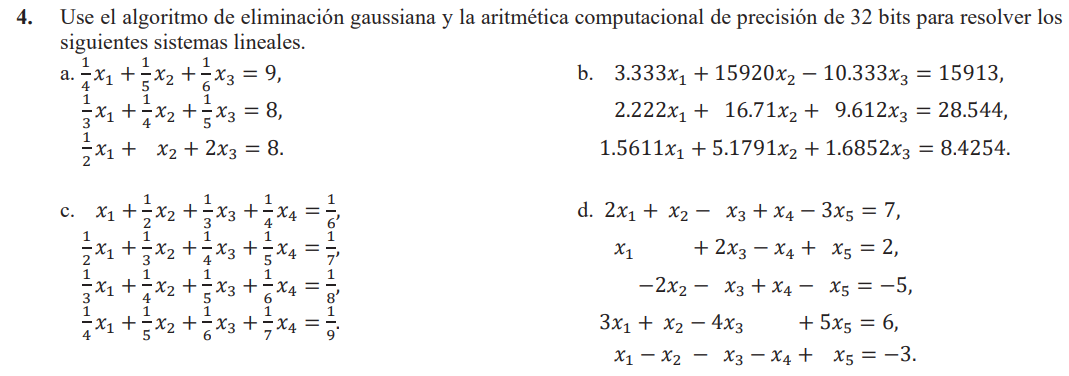
\includegraphics[width=1\textwidth]{./inFiles/Figures/Ej4.png}
\end{figure}

Por código:
\begin{figure}[H]
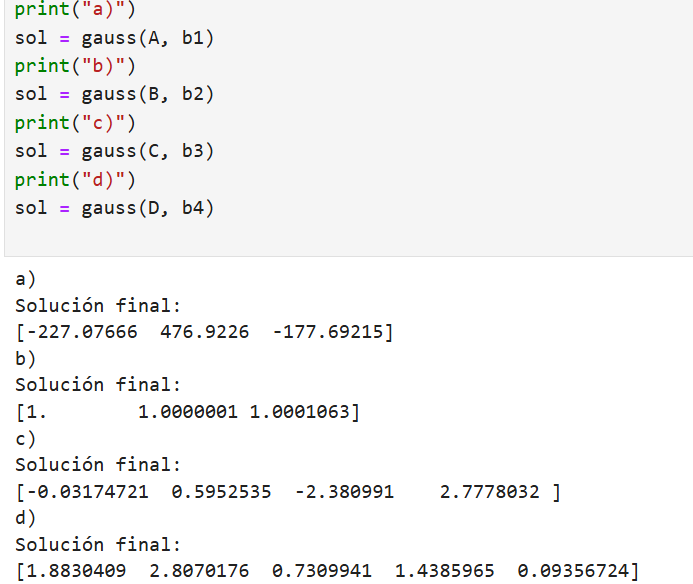
\includegraphics[width=1\textwidth]{./inFiles/Figures/PC4.png}
\end{figure}

A mano:


\textbf{a)}

\[
\begin{bmatrix}
0.25 & 0.2 & 0.16666667 & 9 \\
0.33333334 & 0.25 & 0.2 & 8 \\
0.5 & 1 & 2 & 8 \\
\end{bmatrix}
\]

0.25*F2-0.33333334*F1$\longrightarrow $ F2

-2*F1+F3 $\longrightarrow $ F3

\[
\begin{bmatrix}
0.25 & 0.2 & 0.16666667 & 9 \\
0 & -0.004166668 & -0.005555557 & -1 \\
0 & 0.6 & 1.6666666 & -10 \\
\end{bmatrix}
\]

0.6*F2+0.004166668*F3 $\longrightarrow $ F3

\[
\begin{bmatrix}
0.25 & 0.2 & 0.16666667 & 9 \\
0 & -0.004166668 & -0.005555557 & -1 \\
0 & 0 & 0.003611112 & -0.64166668 \\
\end{bmatrix}
\]

Al hacer la sustitución para atrás obtenemos

$X3 = -177.6922676$   $X2 =476.9229325$  $X1 =-227.0768319$ 

\textbf{b)}

\[
\begin{bmatrix}
3.333 & 15920 & -10.333 & 15913\\
2.222 & 16.71 & 9.612 & 28.544 \\
1.5611 & 5.1791 & 1.6852 & 8.4254\\
\end{bmatrix}
\]

-2.222*F1+3.333*F2  $\longrightarrow $ F2

-1.5611*F1+3.333*F3 $\longrightarrow $ F3

\[
\begin{bmatrix}
3.333 & 15920 & -10.333 & 15913\\
0 & -35318.54557 & 54.996722 & -35263.54885 \\
0 & -24835.45006 & 21.7476179 & -24813.70244\\
\end{bmatrix}
\]

-24835.45006*F2+35318.54557*F3 $\longrightarrow $ F3

\[
\begin{bmatrix}
3.333 & 15920 & -10.333 & 15913\\
0 & -35318.54557 & 54.996722 & -35263.54885 \\
0 & 0 & -597774.1089 & -597773.985\\
\end{bmatrix}
\]

Al hacer la sustitución para atrás obtenemos

$X3 = 0.99999979$   $X2 =0.99999999$  $X1 =1.000047$ 


\textbf{c)}

\[
\begin{bmatrix}
1 & 0.5 & 0.33333334 & 0.25 & 0.16666667 \\
0.5 & 0.33333334 & 0.25 & 0.2 & 0.14285714\\
0.33333334 & 0.25 & 0.2 & 0.16666667 & 0.125\\
0.25 & 0.2 & 0.16666667 & 0.14285714 & 0.11111111\\
\end{bmatrix}
\]

-0.5*F1+F2  $\longrightarrow $ F2

-0.33333334*F1+F3 $\longrightarrow $ F3

-0.25*F1+F4  $\longrightarrow $ F4

\[
\begin{bmatrix}
1 & 0.5 & 0.33333334 & 0.25 & 0.16666667 \\
0 & 0.083333330 & 0.083333335 & 0.075 & 0.059523805\\
0 & 0.083333335 & 0.088888891 & 0.083333338 & 0.06944444\\
0 & 0.075 & 0.083333338 & 0.08035714 & 0.06944444\\
\end{bmatrix}
\]

-0.083333335*F2+0.083333330*F3  $\longrightarrow $ F3

-0.075*F1+0.083333330*F4 $\longrightarrow $ F4

\[
\begin{bmatrix}
1 & 0.5 & 0.33333334 & 0.25 & 0.16666667 \\
0 & 0.083333330 & 0.083333335 & 0.075 & 0.059523805\\
0 & 0 & 0.000462962 & 0.000694444 & 0.000826719\\
0 & 0 & 0.000694444 & 0.001071428 & 0.001322751\\
\end{bmatrix}
\]

-0.000694444*F3+0.000462962*F4 $\longrightarrow $ F4

\[
\begin{bmatrix}
1 & 0.5 & 0.33333334 & 0.25 & 0.16666667 \\
0 & 0.083333330 & 0.083333335 & 0.075 & 0.059523805\\
0 & 0 & 0.000462962 & 0.000694444 & 0.000826719\\
0 & 0 & 0 & 0.000000013 & 0.000000038\\
\end{bmatrix}
\]

Al hacer la sustitución para atrás obtenemos

$X4 = 2.92307692$ $X3 = -2.59890445$   $X2 =0.68242098$  $X1 =-0.03901158$ 


\textbf{d)}

\[
\begin{bmatrix}
2 & 1 & -1 & 1 & -3 & 7\\
1 & 0 & 2 & -1 & 1 & 2\\
0 & -2 & -1 & 1 & -1 & -5\\
3 & 1 & -4 & 0 & 5 & 6\\
1 & -1 & -1 & -1 & 1 & -3\\
\end{bmatrix}
\]

Hacemos algunos cambios de filas
\[
\begin{bmatrix}
1 & 0 & 2 & -1 & 1 & 2\\ 
1 & -1 & -1 & -1 & 1 & -3\\
0 & -2 & -1 & 1 & -1 & -5\\   
2 & 1 & -1 & 1 & -3 & 7\\
3 & 1 & -4 & 0 & 5 & 6\\
\end{bmatrix}
\]

-F1 + F2 $\longrightarrow $ F2

-2F1 + F24$\longrightarrow $ F4

-3F1 + F5 $\longrightarrow $ F5

\[
\begin{bmatrix}
1 & 0 & 2 & -1 & 1 & 2\\ 
0 & -1 & -3 & 0 & 0 & -5\\
0 & -2 & -1 & 1 & -1 & -5\\   
0 & 1 & -5 & 3 & -5 & 3\\
0 & 1 & -10 & 3 & 2 & 0\\
\end{bmatrix}
\]

-2F2 + F3 $\longrightarrow $ F3

F2 + F4 $\longrightarrow $ F4

F2 + F5 $\longrightarrow $ F5

\[
\begin{bmatrix}
1 & 0 & 2 & -1 & 1 & 2\\ 
0 & -1 & -3 & 0 & 0 & -5\\
0 & 0 & 5 & 1 & -1 & 5\\   
0 & 0 & -8 & 3 & -5 & -2\\
0 & 0 & -13 & 3 & 2 & 5\\
\end{bmatrix}
\]

8F3 + 5F4 $\longrightarrow $ F4

13F3 + 5F5 $\longrightarrow $ F5

\[
\begin{bmatrix}
1 & 0 & 2 & -1 & 1 & 2\\ 
0 & -1 & -3 & 0 & 0 & -5\\
0 & 0 & 5 & 1 & -1 & 5\\   
0 & 0 & 0 & 23 & -33 & 30\\
0 & 0 & 0 & 28 & -3 & 40\\
\end{bmatrix}
\]

-28F4 + 23F5 $\longrightarrow $ F5

\[
\begin{bmatrix}
1 & 0 & 2 & -1 & 1 & 2\\ 
0 & -1 & -3 & 0 & 0 & -5\\
0 & 0 & 5 & 1 & -1 & 5\\   
0 & 0 & 0 & 23 & -33 & 30\\
0 & 0 & 0 & 0 & 855 & 80\\
\end{bmatrix}
\]

Al hacer la sustitución para atrás obtenemos

$X5 = 0.093567251$ 

$X4 = 1.43859649$ 

$X3 = 0.73099415$   

$X2 =2.80701755$  

$X1 =1.88304089$ 





\begin{figure}[H]
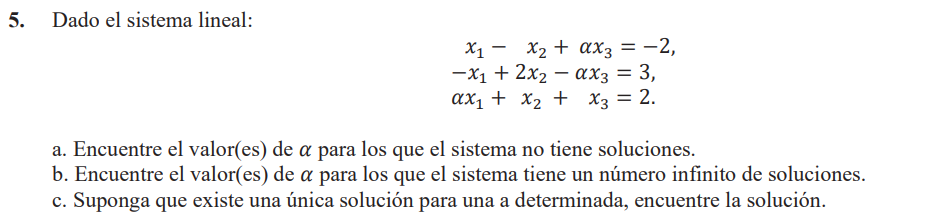
\includegraphics[width=1\textwidth]{./inFiles/Figures/Ej5.png}
\end{figure}

\[
\begin{bmatrix}
1 & -1 & \alpha & -2 \\
-1 & 2 & -\alpha& 3 \\
\alpha & 1 & 1 & 2
\end{bmatrix}
\]

F1+F2 $\longrightarrow $ F2

\[
\begin{bmatrix}
1 & -1 & \alpha & -2 \\
0 & 1 & 0&1 \\
\alpha & 1 & 1 & 2
\end{bmatrix}
\]

-$\alpha$F1+F3 $\longrightarrow $ F3

\[
\begin{bmatrix}
1 & -1 & \alpha & -2 \\
0 & 1 & 0&1 \\
0 & 1+\alpha & 1-\alpha^2 & 2+2\alpha
\end{bmatrix}
\]

Ahora se divide en dos casos cuando $\alpha=0$ o $\alpha\neq 0$ (Porque no se puede multiplicar por 0)

$\alpha=0$

\[
\begin{bmatrix}
1 & -1 & 0 & -2 \\
0 & 1 & 0&1 \\
0 & 1 & 1 & 2
\end{bmatrix}
\]

Obtenemos una única solución donde x2 = 1, x3 = 1 x1 = -1

$\alpha\neq 0$
\[
\begin{bmatrix}
1 & -1 & \alpha & -2 \\
0 & 1 & 0&1 \\
0 & 1+\alpha & 1-\alpha^2 & 2+2\alpha
\end{bmatrix}
\]
Aquí nos damos cuenta que si alpha es -1 tenemos infinitas soluciones porque tendríamos una ecuación menos.


Si alpha es 1 no tenemos solución porque tendríamos en la ultima fila 2x2 = 4 pero en la segunda fila tengo x2 = 1, 
por lo tanto no habría solución.

Y para cualquier otro valor obtendría una única solución.

Ej 
$\alpha=2$
\[
\begin{bmatrix}
1 & -1 & 2 & -2 \\
0 & 1 & 0&1 \\
0 & 3 & -3 & 6
\end{bmatrix}
\]

-3F2+F3 $\longrightarrow $ F3

\[
\begin{bmatrix}
1 & -1 & 2 & -2 \\
0 & 1 & 0&1 \\
0 & 0 & -3 & 3
\end{bmatrix}
\]

Haciendo la substitución para atrás 
$X3 = -1$   $X2 =1$  $X1 =1$ 

\begin{figure}[H]
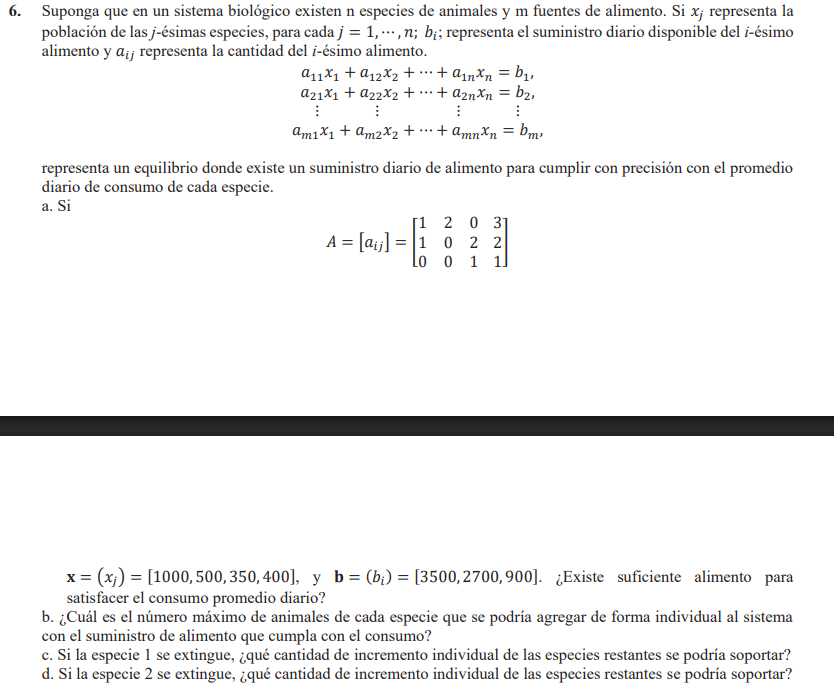
\includegraphics[width=1\textwidth]{./inFiles/Figures/Ej6.png}
\end{figure}


\textbf{a)}

Al reemplazar las x obtengo

\[
\begin{bmatrix}
3200 \\
2500\\
750
\end{bmatrix}
\] 
Y son menores al consumo asi que si se satisface.


\textbf{b)} Para k1 y para los demás, solo que difiere en la posición de ki en la columna(k representa el incremento primera,segunda,... especie)
\[
\begin{bmatrix}
1 & 2 & 0 & 3 \\
1 & 0 & 2 & 2 \\
0 &0 & 1& 1 
\end{bmatrix}
*(
\begin{bmatrix}
1000 \\
500\\
350\\
400
\end{bmatrix}
+
\begin{bmatrix}
k1\\
0\\
0\\
0

\end{bmatrix}
)\leq
\begin{bmatrix}
3500\\
2700\\
900
\end{bmatrix}
\] 
Al operar obtengo
\[
\begin{bmatrix}
k1 \\
k1 \\
k1
\end{bmatrix} \leq 
\begin{bmatrix}
300 \\
200\\
150/0
\end{bmatrix}
\] 

Especie 1 = 200 esp mas

Aquí me da el incremento para cada alimento por lo que eligo el que se adapte a todos.
No considero la ultima porque nos dice que para el alimento en donde se tenga k por 0 se puede incrementar infinitamente los animales porque no consumen dicho alimento.

Para k2

Al operar obtengo
\[
\begin{bmatrix}
k2 \\
k2 \\
k2
\end{bmatrix} \leq 
\begin{bmatrix}
150 \\
200/0\\
150/0
\end{bmatrix}
\] 

Especie 2 = 150 esp mas

Para k3

Al operar obtengo
\[
\begin{bmatrix}
k3 \\
k3 \\
k3
\end{bmatrix} \leq 
\begin{bmatrix}
300/0\\
100\\
150
\end{bmatrix}
\] 

Especie 3 = 100 esp mas

Para k4

Al operar obtengo
\[
\begin{bmatrix}
k4 \\
k4  \\
k4 
\end{bmatrix} \leq 
\begin{bmatrix}
100\\
100\\
150
\end{bmatrix}
\] 

Especie 4 = 100 esp mas

\textbf{c)} Reemplazo primera fila de x por 0 y no analizo k1 porque no existe la especie.
\[
\begin{bmatrix}
1 & 2 & 0 & 3 \\
1 & 0 & 2 & 2 \\
0 &0 & 1& 1 
\end{bmatrix}
*(
\begin{bmatrix}
0 \\
500\\
350\\
400
\end{bmatrix}
+
\begin{bmatrix}
0\\
k2\\
0\\
0

\end{bmatrix}
)\leq
\begin{bmatrix}
3500\\
2700\\
900
\end{bmatrix}
\] 
Al operar obtengo
\[
\begin{bmatrix}
k2 \\
k2 \\
k2
\end{bmatrix} \leq 
\begin{bmatrix}
650\\
1200/0\\
150/0
\end{bmatrix}
\] 

Especie 2 = 650 esp mas

Para k3 

Al operar obtengo
\[
\begin{bmatrix}
k3 \\
k3 \\
k3
\end{bmatrix} \leq 
\begin{bmatrix}
1300/0\\
600\\
150
\end{bmatrix}
\] 

Especie 3 = 150 esp mas

Para k4

Al operar obtengo
\[
\begin{bmatrix}
k4 \\
k4 \\
k4
\end{bmatrix} \leq 
\begin{bmatrix}
433.33\\
600\\
150
\end{bmatrix}
\] 

Especie 4 = 150 esp mas

\textbf{d)} Reemplazo segunda fila de x por 0 y no analizo k2 porque no existe la especie.
\[
\begin{bmatrix}
1 & 2 & 0 & 3 \\
1 & 0 & 2 & 2 \\
0 &0 & 1& 1 
\end{bmatrix}
*(
\begin{bmatrix}
1000 \\
0\\
350\\
400
\end{bmatrix}
+
\begin{bmatrix}
k1\\
0\\
0\\
0

\end{bmatrix}
)\leq
\begin{bmatrix}
3500\\
2700\\
900
\end{bmatrix}
\] 
Al operar obtengo
\[
\begin{bmatrix}
k1 \\
k1 \\
k1
\end{bmatrix} \leq 
\begin{bmatrix}
1300\\
200\\
150/0
\end{bmatrix}
\] 

Especie 1 = 200 esp mas

Para k3 

Al operar obtengo
\[
\begin{bmatrix}
k3 \\
k3 \\
k3
\end{bmatrix} \leq 
\begin{bmatrix}
1300/0\\
100\\
150
\end{bmatrix}
\] 

Especie 3 = 100 esp mas

Para k4

Al operar obtengo
\[
\begin{bmatrix}
k4 \\
k4 \\
k4
\end{bmatrix} \leq 
\begin{bmatrix}
433.33\\
100\\
150
\end{bmatrix}
\] 

Especie 4 = 100 esp mas

\begin{figure}[H]
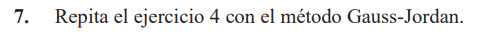
\includegraphics[width=1\textwidth]{./inFiles/Figures/Ej7.png}
\end{figure}


\textbf{a)}

\[
\begin{bmatrix}
0.25 & 0.2 & 0.16666667 & 9 \\
0.33333334 & 0.25 & 0.2 & 8 \\
0.5 & 1 & 2 & 8 \\
\end{bmatrix}
\]

0.25*F2-0.33333334*F1$\longrightarrow $ F2

-2*F1+F3 $\longrightarrow $ F3

\[
\begin{bmatrix}
0.25 & 0.2 & 0.16666667 & 9 \\
0 & -0.004166668 & -0.005555557 & -1 \\
0 & 0.6 & 1.6666666 & -10 \\
\end{bmatrix}
\]

0.6*F2+0.004166668*F3 $\longrightarrow $ F3

\[
\begin{bmatrix}
0.25 & 0.2 & 0.16666667 & 9 \\
0 & -0.004166668 & -0.005555557 & -1 \\
0 & 0 & 0.003611112 & -0.64166668 \\
\end{bmatrix}
\]

F3/0.003611112  $\longrightarrow $ F3

0.005555557*F3 +F2 $\longrightarrow $ F2

-0.16666667*F3+F1  $\longrightarrow $ F1

\[
\begin{bmatrix}
0.25 & 0.2 & 0 & 38.61537853 \\
0 & -0.004166668 & 0 & -1.98717952 \\
0 & 0 & 1 & -177.6922676\\
\end{bmatrix}
\]

F2/-0.004166668  $\longrightarrow $ F3

-0.2*F2+F1  $\longrightarrow $ F1

F1/0.25  $\longrightarrow $ F1

\[
\begin{bmatrix}
1 & 0 & 0 & -227.0768319 \\
0 & 1 & 0 & 476.9229325 \\
0 & 0 & 1 & -177.6922676\\
\end{bmatrix}
\]
\textbf{b)}

\[
\begin{bmatrix}
3.333 & 15920 & -10.333 & 15913\\
2.222 & 16.71 & 9.612 & 28.544 \\
1.5611 & 5.1791 & 1.6852 & 8.4254\\
\end{bmatrix}
\]

-2.222*F1+3.333*F2  $\longrightarrow $ F2

-1.5611*F1+3.333*F3 $\longrightarrow $ F3

\[
\begin{bmatrix}
3.333 & 15920 & -10.333 & 15913\\
0 & -35318.54557 & 54.996722 & -35263.54885 \\
0 & -24835.45006 & 21.7476179 & -24813.70244\\
\end{bmatrix}
\]

-24835.45006*F2+35318.54557*F3 $\longrightarrow $ F3

\[
\begin{bmatrix}
3.333 & 15920 & -10.333 & 15913\\
0 & -35318.54557 & 54.996722 & -35263.54885 \\
0 & 0 & -597774.1089 & -597773.985\\
\end{bmatrix}
\]

F3/-597774.1089  $\longrightarrow $ F3

10.333*F3+F1  $\longrightarrow $ F1

-54.996722*F3+F2 $\longrightarrow $ F2

\[
\begin{bmatrix}
3.333 & 15920 & 0 & 15923.333\\
0 & -35318.54557 & 0 & -35318.54556 \\
0 & 0 & 1 & 0.99999979\\
\end{bmatrix}
\]

F2/-35318.54557 $\longrightarrow $ F2

15920*F2+F1 $\longrightarrow $ F1

F1/3.333 $\longrightarrow $ F1
\[
\begin{bmatrix}
1 & 0 & 0 & 1.000047\\
0 & 1 & 0 & 0.99999999 \\
0 & 0 & 1 & 0.99999979\\
\end{bmatrix}
\]

\textbf{c)}

\[
\begin{bmatrix}
1 & 0.5 & 0.33333334 & 0.25 & 0.16666667 \\
0.5 & 0.33333334 & 0.25 & 0.2 & 0.14285714\\
0.33333334 & 0.25 & 0.2 & 0.16666667 & 0.125\\
0.25 & 0.2 & 0.16666667 & 0.14285714 & 0.11111111\\
\end{bmatrix}
\]

-0.5*F1+F2  $\longrightarrow $ F2

-0.33333334*F1+F3 $\longrightarrow $ F3

-0.25*F1+F4  $\longrightarrow $ F4

\[
\begin{bmatrix}
1 & 0.5 & 0.33333334 & 0.25 & 0.16666667 \\
0 & 0.083333330 & 0.083333335 & 0.075 & 0.059523805\\
0 & 0.083333335 & 0.088888891 & 0.083333338 & 0.06944444\\
0 & 0.075 & 0.083333338 & 0.08035714 & 0.06944444\\
\end{bmatrix}
\]

-0.083333335*F2+0.083333330*F3  $\longrightarrow $ F3

-0.075*F1+0.083333330*F4 $\longrightarrow $ F4

\[
\begin{bmatrix}
1 & 0.5 & 0.33333334 & 0.25 & 0.16666667 \\
0 & 0.083333330 & 0.083333335 & 0.075 & 0.059523805\\
0 & 0 & 0.000462962 & 0.000694444 & 0.000826719\\
0 & 0 & 0.000694444 & 0.001071428 & 0.001322751\\
\end{bmatrix}
\]

-0.000694444*F3+0.000462962*F4 $\longrightarrow $ F4

\[
\begin{bmatrix}
1 & 0.5 & 0.33333334 & 0.25 & 0.16666667 \\
0 & 0.083333330 & 0.083333335 & 0.075 & 0.059523805\\
0 & 0 & 0.000462962 & 0.000694444 & 0.000826719\\
0 & 0 & 0 & 0.000000013 & 0.000000038\\
\end{bmatrix}
\]


F4/0.000000013 $\longrightarrow $ F4

-0.000694444*F4+F3 $\longrightarrow $ F3

-0.075*F4+F2 $\longrightarrow $ F2

-0.25*F4+F1 $\longrightarrow $ F1

\[
\begin{bmatrix}
1 & 0.5 & 0.33333334 & 0 & -0.56410256\\
0 & 0.083333330 & 0.083333335 & 0 & -0.15970696\\
0 & 0 & 0.000462962 & 0 & -0.001203194\\
0 & 0 & 0 & 1 & 2.92307692\\
\end{bmatrix}
\]

F3/0.000462962 $\longrightarrow $ F3

-0.083333335*F3 + F2$\longrightarrow $ F2

-0.33333334*F3 + F1$\longrightarrow $ F1

\[
\begin{bmatrix}
1 & 0.5 & 0 & 0 & -0.56410256\\
0 & 0.083333330 & 0 & 0 & -0.15970696\\
0 & 0 & 1 & 0 & -2.59890445\\
0 & 0 & 0 & 1 & 2.92307692\\
\end{bmatrix}
\]

F2/0.083333330 $\longrightarrow $ F2
-0.5*F2+F1 $\longrightarrow $ F1

\[
\begin{bmatrix}
1 & 0 & 0 & 0 & -0.03901158\\
0 & 1 & 0 & 0 & 0.68242098\\
0 & 0 & 1 & 0 & -2.59890445\\
0 & 0 & 0 & 1 & 2.92307692\\
\end{bmatrix}
\]


\textbf{d)}

\[
\begin{bmatrix}
2 & 1 & -1 & 1 & -3 & 7\\
1 & 0 & 2 & -1 & 1 & 2\\
0 & -2 & -1 & 1 & -1 & -5\\
3 & 1 & -4 & 0 & 5 & 6\\
1 & -1 & -1 & -1 & 1 & -3\\
\end{bmatrix}
\]

Hacemos algunos cambios de filas
\[
\begin{bmatrix}
1 & 0 & 2 & -1 & 1 & 2\\ 
1 & -1 & -1 & -1 & 1 & -3\\
0 & -2 & -1 & 1 & -1 & -5\\   
2 & 1 & -1 & 1 & -3 & 7\\
3 & 1 & -4 & 0 & 5 & 6\\
\end{bmatrix}
\]

-F1 + F2 $\longrightarrow $ F2

-2F1 + F24$\longrightarrow $ F4

-3F1 + F5 $\longrightarrow $ F5

\[
\begin{bmatrix}
1 & 0 & 2 & -1 & 1 & 2\\ 
0 & -1 & -3 & 0 & 0 & -5\\
0 & -2 & -1 & 1 & -1 & -5\\   
0 & 1 & -5 & 3 & -5 & 3\\
0 & 1 & -10 & 3 & 2 & 0\\
\end{bmatrix}
\]

-2F2 + F3 $\longrightarrow $ F3

F2 + F4 $\longrightarrow $ F4

F2 + F5 $\longrightarrow $ F5

\[
\begin{bmatrix}
1 & 0 & 2 & -1 & 1 & 2\\ 
0 & -1 & -3 & 0 & 0 & -5\\
0 & 0 & 5 & 1 & -1 & 5\\   
0 & 0 & -8 & 3 & -5 & -2\\
0 & 0 & -13 & 3 & 2 & 5\\
\end{bmatrix}
\]

8F3 + 5F4 $\longrightarrow $ F4

13F3 + 5F5 $\longrightarrow $ F5

\[
\begin{bmatrix}
1 & 0 & 2 & -1 & 1 & 2\\ 
0 & -1 & -3 & 0 & 0 & -5\\
0 & 0 & 5 & 1 & -1 & 5\\   
0 & 0 & 0 & 23 & -33 & 30\\
0 & 0 & 0 & 28 & -3 & 40\\
\end{bmatrix}
\]

-28F4 + 23F5 $\longrightarrow $ F5

\[
\begin{bmatrix}
1 & 0 & 2 & -1 & 1 & 2\\ 
0 & -1 & -3 & 0 & 0 & -5\\
0 & 0 & 5 & 1 & -1 & 5\\   
0 & 0 & 0 & 23 & -33 & 30\\
0 & 0 & 0 & 0 & 855 & 80\\
\end{bmatrix}
\]

F5/855 $\longrightarrow $ F5

-F5+F1$\longrightarrow $ F1

F5+F3$\longrightarrow $ F3

33F5+F4$\longrightarrow $ F4

\[
\begin{bmatrix}
1 & 0 & 2 & -1 & 0 & 1.9064327\\ 
0 & -1 & -3 & 0 & 0 & -5\\
0 & 0 & 5 & 1 & 0 & 5.093567251\\   
0 & 0 & 0 & 23 & 0 & 33.08771938\\
0 & 0 & 0 & 0 & 1 & 0.093567251\\
\end{bmatrix}
\]

F4/23 $\longrightarrow $ F4

F4+F1$\longrightarrow $ F1

-F4+F3$\longrightarrow $ F3

\[
\begin{bmatrix}
1 & 0 & 2 & 0 & 0 & 3.34502919\\ 
0 & -1 & -3 & 0 & 0 & -5\\
0 & 0 & 5 & 0 & 0 & 3.65497076\\   
0 & 0 & 0 & 1 & 0 & 1.43859649\\
0 & 0 & 0 & 0 & 1 & 0.093567251\\
\end{bmatrix}
\]

F3/5 $\longrightarrow $ F3

3F3+F2$\longrightarrow $ F2

-2*F3+F1$\longrightarrow $ F1

\[
\begin{bmatrix}
1 & 0 & 0 & 0 & 0 & 1.88304089\\ 
0 & 1 & 0 & 0 & 0 & 2.80701755\\
0 & 0 & 1 & 0 & 0 & 0.73099415\\   
0 & 0 & 0 & 1 & 0 & 1.43859649\\
0 & 0 & 0 & 0 & 1 & 0.093567251\\
\end{bmatrix}
\]





\vspace{0.5cm}
\renewcommand{\refname}{\MakeUppercase{REFERENCIAS}}
\bibliographystyle{IEEEtran}
\bibliography{inFiles/References/references.bib}

\end{document}
